

\tikzset{every picture/.style={line width=0.75pt}} %set default line width to 0.75pt

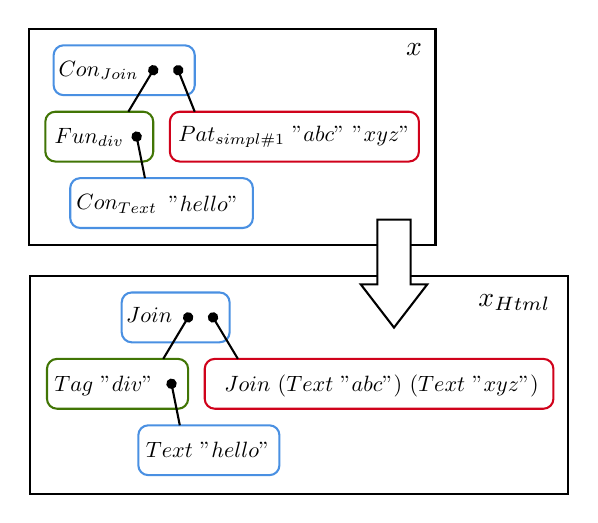
\begin{tikzpicture}[x=0.75pt,y=0.75pt,yscale=-0.8,xscale=0.8]
%uncomment if require: \path (0,440.8571319580078); %set diagram left start at 0, and has height of 440.8571319580078

%Rounded Rect [id:dp4443669613398804]
\draw  [color={rgb, 255:red, 208; green, 2; blue, 27 }  ,draw opacity=1 ] (100,66) .. controls (100,62.69) and (102.69,60) .. (106,60) -- (244,60) .. controls (247.31,60) and (250,62.69) .. (250,66) -- (250,84) .. controls (250,87.31) and (247.31,90) .. (244,90) -- (106,90) .. controls (102.69,90) and (100,87.31) .. (100,84) -- cycle ;

%Rounded Rect [id:dp2445219502409255]
\draw  [color={rgb, 255:red, 65; green, 117; blue, 5 }  ,draw opacity=1 ] (25,66) .. controls (25,62.69) and (27.69,60) .. (31,60) -- (84,60) .. controls (87.31,60) and (90,62.69) .. (90,66) -- (90,84) .. controls (90,87.31) and (87.31,90) .. (84,90) -- (31,90) .. controls (27.69,90) and (25,87.31) .. (25,84) -- cycle ;
%Rounded Rect [id:dp9597491817026895]
\draw  [color={rgb, 255:red, 74; green, 144; blue, 226 }  ,draw opacity=1 ] (30,26) .. controls (30,22.69) and (32.69,20) .. (36,20) -- (109,20) .. controls (112.31,20) and (115,22.69) .. (115,26) -- (115,44) .. controls (115,47.31) and (112.31,50) .. (109,50) -- (36,50) .. controls (32.69,50) and (30,47.31) .. (30,44) -- cycle ;

%Straight Lines [id:da4767955800901629]
\draw    (90,35) -- (75,60) ;

\draw [shift={(90,35)}, rotate = 120.96] [color={rgb, 255:red, 0; green, 0; blue, 0 }  ][fill={rgb, 255:red, 0; green, 0; blue, 0 }  ][line width=0.75]      (0, 0) circle [x radius=2.5, y radius=2.5]   ;
%Straight Lines [id:da737226333560641]
\draw    (105,35) -- (115,60) ;

\draw [shift={(105,35)}, rotate = 68.2] [color={rgb, 255:red, 0; green, 0; blue, 0 }  ][fill={rgb, 255:red, 0; green, 0; blue, 0 }  ][line width=0.75]      (0, 0) circle [x radius=2.5, y radius=2.5]   ;
%Rounded Rect [id:dp9147190163305616]
\draw  [color={rgb, 255:red, 74; green, 144; blue, 226 }  ,draw opacity=1 ] (40,106) .. controls (40,102.69) and (42.69,100) .. (46,100) -- (144,100) .. controls (147.31,100) and (150,102.69) .. (150,106) -- (150,124) .. controls (150,127.31) and (147.31,130) .. (144,130) -- (46,130) .. controls (42.69,130) and (40,127.31) .. (40,124) -- cycle ;
%Straight Lines [id:da2709254544231703]
\draw    (80,75) -- (85,100) ;

\draw [shift={(80,75)}, rotate = 78.69] [color={rgb, 255:red, 0; green, 0; blue, 0 }  ][fill={rgb, 255:red, 0; green, 0; blue, 0 }  ][line width=0.75]      (0, 0) circle [x radius=2.5, y radius=2.5]   ;

%Shape: Rectangle [id:dp9665612509271984]
\draw   (15,10) -- (260,10) -- (260,140) -- (15,140) -- cycle ;

%Rounded Rect [id:dp8911386762864086]
\draw  [color={rgb, 255:red, 208; green, 2; blue, 27 }  ,draw opacity=1 ] (121,214.86) .. controls (121,211.54) and (123.69,208.86) .. (127,208.86) -- (325,208.86) .. controls (328.31,208.86) and (331,211.54) .. (331,214.86) -- (331,232.86) .. controls (331,236.17) and (328.31,238.86) .. (325,238.86) -- (127,238.86) .. controls (123.69,238.86) and (121,236.17) .. (121,232.86) -- cycle ;

%Rounded Rect [id:dp28519778620668634]
\draw  [color={rgb, 255:red, 65; green, 117; blue, 5 }  ,draw opacity=1 ] (26,214.86) .. controls (26,211.54) and (28.69,208.86) .. (32,208.86) -- (105,208.86) .. controls (108.31,208.86) and (111,211.54) .. (111,214.86) -- (111,232.86) .. controls (111,236.17) and (108.31,238.86) .. (105,238.86) -- (32,238.86) .. controls (28.69,238.86) and (26,236.17) .. (26,232.86) -- cycle ;
%Rounded Rect [id:dp42988108204777453]
\draw  [color={rgb, 255:red, 74; green, 144; blue, 226 }  ,draw opacity=1 ] (71,174.86) .. controls (71,171.54) and (73.69,168.86) .. (77,168.86) -- (130,168.86) .. controls (133.31,168.86) and (136,171.54) .. (136,174.86) -- (136,192.86) .. controls (136,196.17) and (133.31,198.86) .. (130,198.86) -- (77,198.86) .. controls (73.69,198.86) and (71,196.17) .. (71,192.86) -- cycle ;
%Straight Lines [id:da7584739344782256]
\draw    (111,183.86) -- (96,208.86) ;

\draw [shift={(111,183.86)}, rotate = 120.96] [color={rgb, 255:red, 0; green, 0; blue, 0 }  ][fill={rgb, 255:red, 0; green, 0; blue, 0 }  ][line width=0.75]      (0, 0) circle [x radius=2.5, y radius=2.5]   ;
%Straight Lines [id:da9525312529597059]
\draw    (126,183.86) -- (141,208.86) ;

\draw [shift={(126,183.86)}, rotate = 59.04] [color={rgb, 255:red, 0; green, 0; blue, 0 }  ][fill={rgb, 255:red, 0; green, 0; blue, 0 }  ][line width=0.75]      (0, 0) circle [x radius=2.5, y radius=2.5]   ;
%Rounded Rect [id:dp10243358267189961]
\draw  [color={rgb, 255:red, 74; green, 144; blue, 226 }  ,draw opacity=1 ] (81,254.86) .. controls (81,251.54) and (83.69,248.86) .. (87,248.86) -- (160,248.86) .. controls (163.31,248.86) and (166,251.54) .. (166,254.86) -- (166,272.86) .. controls (166,276.17) and (163.31,278.86) .. (160,278.86) -- (87,278.86) .. controls (83.69,278.86) and (81,276.17) .. (81,272.86) -- cycle ;

%Straight Lines [id:da01173054188383471]
\draw    (101,223.86) -- (106,248.86) ;

\draw [shift={(101,223.86)}, rotate = 78.69] [color={rgb, 255:red, 0; green, 0; blue, 0 }  ][fill={rgb, 255:red, 0; green, 0; blue, 0 }  ][line width=0.75]      (0, 0) circle [x radius=2.5, y radius=2.5]   ;

%Shape: Rectangle [id:dp5499992274881935]
\draw   (16,158.86) -- (340,158.86) -- (340,290) -- (16,290) -- cycle ;

%Down Arrow [id:dp3191824787828028]
\draw  [fill={rgb, 225:red, 225; green, 225; blue, 225 }  ,fill opacity=1 ] (215,164) -- (225,164) -- (225,125) -- (245,125) -- (245,164) -- (255,164) -- (235,190) -- cycle ;

% Text Node
\draw (175,75) node [scale=0.8]  {$Pat_{simpl\#1}\ "abc"\ "xyz"$};
% Text Node
\draw (120.5,115.5) node  [scale=0.8] {$"hello"$};
% Text Node
\draw (51.5,75.5) node  [scale=0.8] {$Fun_{div}$};
% Text Node
\draw (57,35) node  [scale=0.8] {$Con_{Join}$};
% Text Node
\draw (68,115.5) node  [scale=0.8] {$Con_{Text}$};
% Text Node
\draw (62.5,225) node  [scale=0.8] {$Tag\ "div"\ $};
% Text Node
\draw (123,263.36) node  [scale=0.8] {$Text\ "hello"$};
% Text Node
\draw (87.5,182.36) node  [scale=0.8] {$Join$};
% Text Node
\draw (227.5,225) node  [scale=0.8] {$Join\ (Text\ "abc")\ (Text\ "xyz")$};
% Text Node
\draw (247,22.5) node [scale=1]  {$x$};
% Text Node
\draw (307.5,175) node [scale=1]  {$\llbracket x\rrbracket _{Html}$};


\end{tikzpicture}
